\section{Introduction}

Unlike nodes in the Internet, cellular networks perform robust
authentication and network access control of all user devices on the
network. This control allows for cellular networks to provide tighter
guarantees on end-to-end quality of service and track each user's
consumption. These access logs are primarily maintained for the
purposes of billing, but also serve an important role to law
enforcement. Traditional telecommunications companies (telcos)
completely control this authentication and billing management within
their own centralized IT systems, known as the network core.

Community cellular networks are full stack cellular networks, using
the same protocols and user devices (cellphones) as national carriers,
but scoped for small rural communities where national carriers are not
incentivized to deploy their own
infrastructure.\cite{Heimerllongitudinalstudylocal2015} Due to their
rural nature, community cellular networks often cope with a slow and
intermittent backhaul connection between the edge community and the
network core. Assumptions of reliable connectivity between the cell
tower and the network core often break down in remote rural areas, and
standard approaches requiring updates to shared subscriber state in
the core do not allow the network to function when backhaul is down.
Such ``disconnected operation'' is highly desireable in rural
communities and disaster scenarios, where the ability to make a call
to a doctor in town or local emergency responders could be lifesaving.

Furthermore, community cellular networks face everyday challenges in
coordinating operation between a large number of small independent
communities. Local communities in the developing world have their own
local governance structures and network maintainers, but often want to
coordinate operation with other communities in the region to maximize
coverage, allow roaming, and make the sum of all networks more useful
for all the community members. This requires a protocol for
synchronizing network core state between the different communities,
and is complicated by the possibility that a user's particular home
community could go offline at any time (a contingency that traditional
telcos do not have to address).

My research is currently addressing both of these issues through the
development of an LTE packet core optimized for rural community
cellular networks. At the core of such a system is a distributed data
structure allowing both \emph{partioned operation} when a community is
offline and \emph{secure coordination} between independent communities.

\section{Approach}

My project combines the power of conflict free replicated data types
(CRDT)s for strong eventual consistency with a backing secure
distributed ledger for distributed coordination. Individual nodes
collect and batch signed state updates locally in a manner consistent
with CRDT principles, and then disseminate them to a backing secure
distributed ledger when they are online. This provides the following
capabilities distinctly applicable to rural community cellular networks

\begin{itemize}
\item Distributed global knowledge of transaction history to allow
  networks to manage the risk of serving any given user when offline.
\item Cryptographic assurance from the host network and each user that
  offline transactions are accurately recorded.
\item Consistent network core state at all times, with bounded
  convergence to the accurate omniscient state.
\item Straightforward procedures for admitting new network operators
  and users to the network, with codable and enforceable policies to
  govern participant behavior on the network.
\item Replication of data and resilience to failures of individual
  community nodes.
\end{itemize}

\subsection{CRDT}
Conflict-Free Replicated Data Types are a class of data types which
have been shown to provide firm guarantees of Strong Eventual
Consistency.\cite{ShapiroConflictfreereplicateddata2011} A simple
example of a CRDT is a counter implementation, where instead of
storing the current value of the counter, the data structure tracks
individual increments and decrements. These same principles can be
applied to much more complicated data types, including nested and
structured data like JSON, while maintaining the same strong eventual
consistency guarantees.\cite{KleppmannConflictFreeReplicatedJSON2017}

New databases exist based on CRDTs designed to allow hyper-scale web
services spread across a wide geographic area to respond quickly to
queries where having the exact most up to date data is not essential
and the connection to other database replicas may be
unreliable.\cite{DatanetNewCRDT16} These databases provide a guarantee
that strong consistency can be achieved within a finite time window as
soon as connectivity is restored. As far as I have found, all current
implementations assume benign nodes and are optimized for performance
in a data center and web services context. While they tolerate
partitioned operation, they do not provide security guarantees towards
the accuracy and validity of the partitioned data in the presence of
malevolent actors.

\subsection{Secure Distributed Ledgers}
Colloquially referred to as ``blockchains,'' secure distributed
ledgers allow for nodes in a network to efficiently share a view of
global state in a completely distributed manner, without a trusted
intermediary, and in a way tolerant to failure and compromise of
individual nodes.\cite{BabuBlockchainTelco2016} Secure distributed
ledgers are most famous for their applications in crypto-currencies,
but the same techniques can be brought to bear in the context of
tracking any kind of centralized data shared between independent
actors. In the context of community networking, these ledgers
facilitate independent communities in a region banding together into a
large federated service provider with transparent roaming between the
communities.

\subsection{System Architecture}
My prototype implements a CRDT update based state store on top of a
distributed ledger. The system uses the Hyperledger fabric framework
(https://github.com/hyperledger) to instantiate a private ledger. I
selected a private ledger architecture given that the local
communities have established (although loose) relationships and can
identify new community networks for admission to the ledger. In
contrast to true public ledgers in cryptocurrencies like Bitcoin or
Etherium, using a private ledger allows the system to avoid the
necessity of an expensive proof of work based consensus and ordering
mechanism. This is crucial for rural community networks in developing
regions where power often comes from generators or solar
panels. Nothing in the system architecture prevents it from being
implemented on a public ledger in the future as low power distributed
consensus protocols like proof of stake or proof of elapsed time
mature.

A Hyperledger peer is deployed as a container to each community
network, handling synchronization of the local network state to the
global ledger when the network is online. All of the peers run an
agreed upon common ``chaincode'' which codifies the rules of
interacting with the network. My implemented chaincode validates each
CRDT update, checks that it is unique, and appends it to the
appropriate CRDT record. In the Hyperledger private blockchain
framework each transaction is validated by endorsing peers in the
community, ensuring that peers have checked and agree upon the
validity of each transaction before it is committed.

Records are organized per user, with each subscriber of the network
having their own account and own history of transactions. Subscribers
first register with the network from their home communities, recording
their subscriber ID and public key. This public key is validated
against all of their signed transactions and as a part of the
connection handshake when they join the network.

As users interact with the local community network, they generate
usage entries detailing the amount of network resources
consumed. These entries are signed by both the user and the network,
and each holds a copy of the cosigned update in case the network is
offline. This ensures that at least one party is incentivized to
report all transactions that occur offline. Users are strongly
incentivized to report any additions or credit purchased, while the
network is strongly incentivized to report all usage to bill users for
their consumed network resources.

My prototype implements these signatures as a fake symmetric key
validation (simply checking that the registered key string is present)
to aid debugging for now, but is easily extensible to strong
cryptographic signatures.

\begin{figure*}[t]
  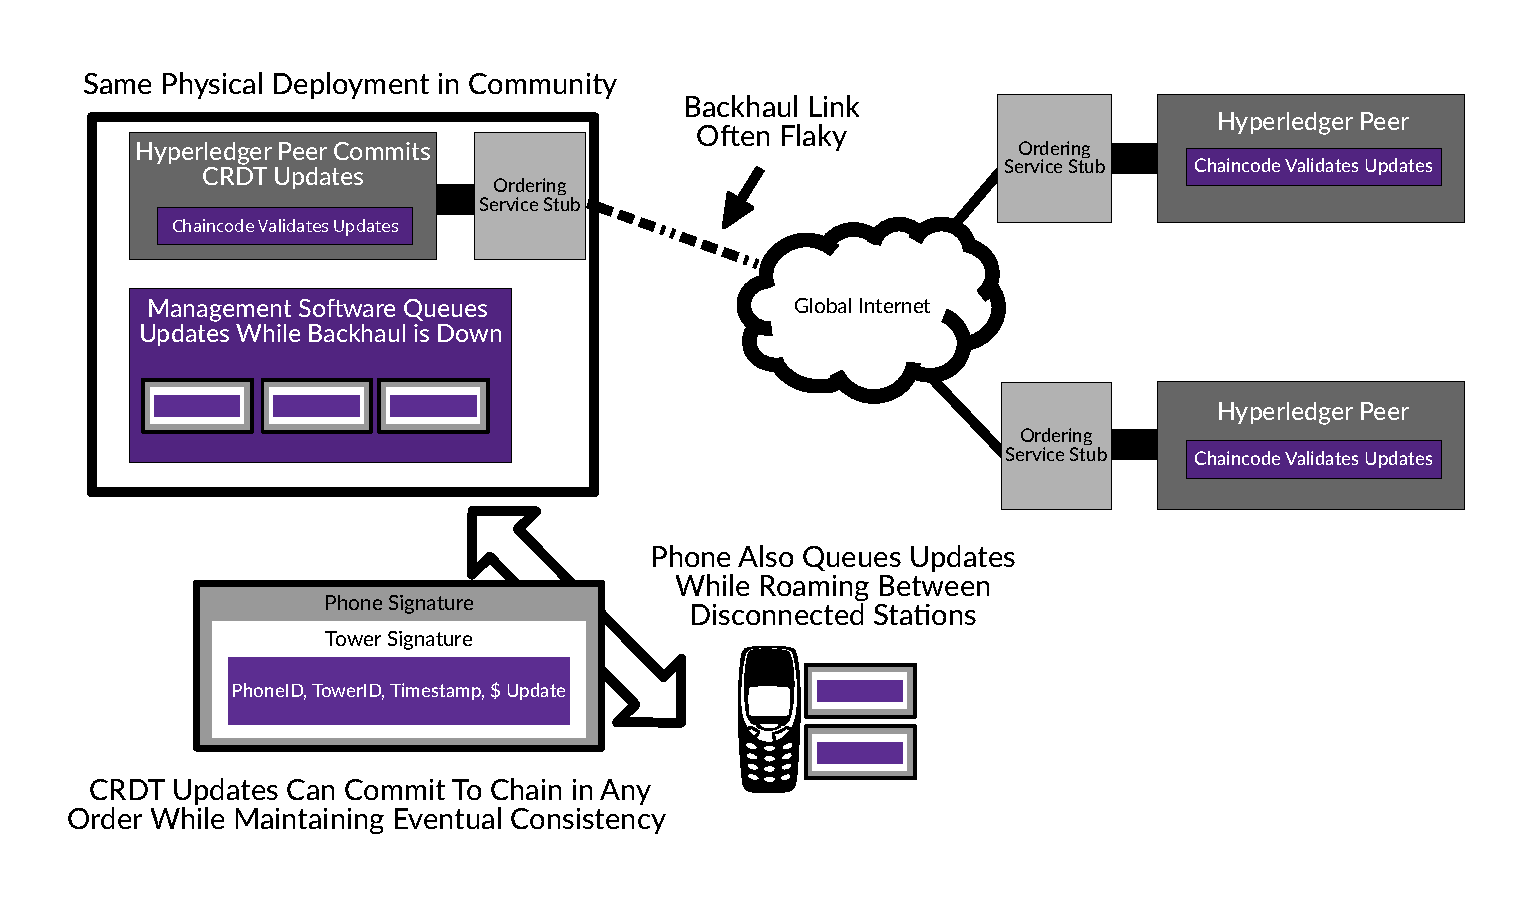
\includegraphics[width=\textwidth]{system-block-diagram}
  \caption{System block diagram showing the updates shared between the
    network and the phone, the station queue manager, and the
    Hyperledger network.}
\end{figure*}

\section{Related Work}
Many high level whitepapers cover the ``opportunities'' for
blockchains in
telecommunications\cite{BabuBlockchainTelco2016}\cite{BubleyBlockchainTelecomsIndustry2017}\cite{BaeOperatingmiddledigital},
but they seem to all be abstract consulting reports driven by
blockchain hype. Furthermore, these reports emphasize concepts from
public blockchains, assuming that the parties involved are well
connected to the global internet, have reliable power, and have
available computing power to perform open distributed consensus. This
work addresses an application of distributed ledgers with a different
set of operational assumptions. There is one key academic paper by
Jover and Lackey\cite{JoverdHSSdistributedPeertoPeer2016a} which
explores building a Home Subscriber Server on a distributed ledger,
but it does not address intermittent backhaul and is only concerned
with user authentication, not user resource tracking as required to
implement a fully functioning network core. My work extends the
concepts covered by Jover and Lackey to provide the functionality
required for a region of rural telcos to coordinate seamless roaming
and billing between networks, even when individual networks are
islanded from the rest of the region. Addressing operation with
unreliable backhaul requires non-trivial changes to the structure of
the data stored on the ledger.

Leveraging existing concepts from theoretical
CRDTs\cite{ShapiroConflictfreereplicateddata2011}, this work presents
a novel CRDT based data storage architecture where individual updates
are signed and cached by users and the network before being
consolidated in a global ledger. I have not found another example of a
distributed co-signed CRDT, although the principle of co-signing is
well established as a means to secure multiparty contracts in a
distributed ledger.

The approach taken here makes a different set of tradeoffs to achieve
distinct end goals from existing CRDT database
implementations.\cite{DatanetNewCRDT16} Datanet uses CRDTs to enable
multi-homed web services over a wide region to simultaneously serve
queries without requiring backend ordering and consensus before
serving a response. My prototype system incurrs additional overhead
compared to datanet by maintaining global state in a secure ledger as
compared to a traditional distributed filesystem, but this model
better maps to the independent governance models of rural community
networks. Using a distributed ledger provides the system resilience to
bad actors or the compromise of one community's infrastructure. 

\section{Implementation}

Over the quarter I have successfully setup a Hyperledger fabric
development environment, developed the necessary chaincode to
validate, commint, and query the CRDT updates, and tested the
chaincode in a Hyperledger network running in containers on my
personal computer. I also developed a local queuing component, the
station queue manager, in javascript/node.js which communicates with
the Hyperledger peer to upload updates when online and store updates
in local memory when the backhaul connection has been interrupted.

\subsection{Chaincode}

In the Hyperledger framework, chaincode is the logic enforcing code
run by each member of the network to validate and enforce
transactions. Results of the chaincode run are compared by the peers
and used to decide what information is added or modified in the shared
ledger. Chaincodes can also be called from other chaincode executions,
allowing chaincode programs to be composed of many components with
state stored in the shared ledger. Hyperledger supports chaincode
development in golang, allowing the chaincode to express the full
range of concepts expressable in this fully featured language. It
provides primitives that can be called from within a chaincode program
to query and update ledger state. Chaincodes are only permitted to
directly query and modify their own pieces of state, but can interact
with other state through composed calls to other chaincodes.

My prototype system implements 4 chaincode functions in two
chaincodes. The first chaincode handles user accounts, and has two
functions to add and query users in the system. The first function
allows registration of new users, appending new user accounts to the
shared ledger. The code validates that the account records are well
formed and that only one public key is registered for each user. The
second allows any user to query for the public key of any other user
for use in transaction validation. This chaincode is used both by the
basestation to authenticate users for network access and by the update
chaincode to validate the signatures in each CRDT record.

The second chaincode manages the CRDT for each registered user, and
also has two functions. The first function allows for querying the
current state of the CRDT for any particular user. This is implemented
as an O(N) scan over the user's datafile to accumulate all CRDT
records for the user. This is not as inefficient as it sounds because
the data is organized contiguously for each user. Future optimizations
could make use of more complicated data structures and checkpointing
to increase performance in a long-running system. The second function
is the most complicated, and supports adding new CRDT records to a
user's history. This function looks up the account public keys for the
user and the tower involved in the record and validates their
signatures on the update. Once validated, it checks that the record
has not been added before, and only then commits the record to the
user's CRDT.

\subsection{Station Queue Manager}

The current station queue manager serves as a proof of concept
prototype to evaluate the performance of the system, accepting query
and update requests from the test client via a basic REST api with
HTTP transport. The queue manager communicates with the Hyperledger
peer via protobuf over GRPC (abstracted by the Hyperledger fabric
sdk). After receiving a request it firsts validates the request
against the known ledger state at the local peer, even when the
network is offline. This allows the queue to save storage space by
discarding invalid updates early and save bandwidth on the constrained
backhaul uplink. Once locally validated, if online the update is sent
to the network for global verification and ordering, and if offline
the update is queued for a future upload. While the current
implementation was sufficient for basic system testing, it lacks
durability features like a persistent on-disk datastore and security
features like https transport and robust access control that would be
required in a real deployment system.

\subsection{Test Client}

To test system performance I also leveraged javascript running in
node.js to develop an automated traffic generator to emulate queries
from the cell network core and the user's phone. The generator
supports generating a variable number of client http requests per
second, targeting both queries of current state and updates to the
database. Discussion of these test results and detailed evaluation
information follows in section \ref{evaluation}.

\section{Evaluation} \label{evaluation}

I plan to evaluated my system across two classes of requirements:
``absolute requirements'' and ``performance requirements''. Absolute
requirements are either met or not met by the system. I evaluated
these requirements through the construction of test cases for each one
and report on if my constructed prototype meets or does not meet each
requirement test.

Currently the only absolute requirements are:
\begin{enumerate}
\item The system must be deployable on a community network basestation
  with 8GB ram, a single quad core processor, and a solid state disk.
\item The system must support offline operation.
\item The system must maintain strong eventual consistency at all
  times under byzantine failure.
\end{enumerate}

I validated requirement (1) by testing my system on a single laptop
computer of comparable performance to a community network
basestation. While the laptop had 16GB of ram, I validated that the
local components never took more than 4GB of memory while running. I
validated requirement (2) by modifying the queue manager to emulate
offline operation. In a deployment scenario I will evaluate this by
physically removing the backhaul connection, but did not have an
immediate way to achieve this in my local test setup for the class
project. I have not yet explicitly validated requirement (3), but
believe it to be true by design through use of the Hyperledger
Framework and the underlying guarantees that it provides.

Performance requirements are related to the performance of my system
implementation and the way the system scales with additional
demand. Performance requirements depend on the amount and
characteristics of traffic, and I evaluated them through measurements
at multiple traffic magnitudes to determine the trend in performance
as traffic/demand increases where relevant.

I gathered the measurements with docker utilization statistics
reported for CPU, Memory, Network, and Disk, and through traces of the
active network traffic during transactions with Wireshark. I measured
the following performance metrics with simulated traffic on a dual
core (hyperthreaded) development machine with 16GB of ram and a solid
state disk:
\begin{itemize}
\item CPU utilization trend peak/avg
\item RAM utilization trend peak/avg
\item Disk io throughput trend peak/avg
\item Disk utilization per transaction
\item Network traffic per transaction
\item Maximum steady state number of updates processed per second
\end{itemize}

On my SSD based machine, the updates appeared to be compute bound,
with little pressure on disk i/o throughput. Hyperledger appeared to
intelligently cache data in memory, only writing to disk when
required. Due to the relatively small size of the individual updates
it appeared they would batch and be flushed as one burst
operation. This was difficult to measure precisely in my test rig due
to background processes and other noise. I was able to measure disk
I/O total per update though, with each update requiring on average
300KB of I/O. The total disk utilization per transaction was much
lower though, with each transaction compressed taking only a few KB.

\begin{figure}[t] 
  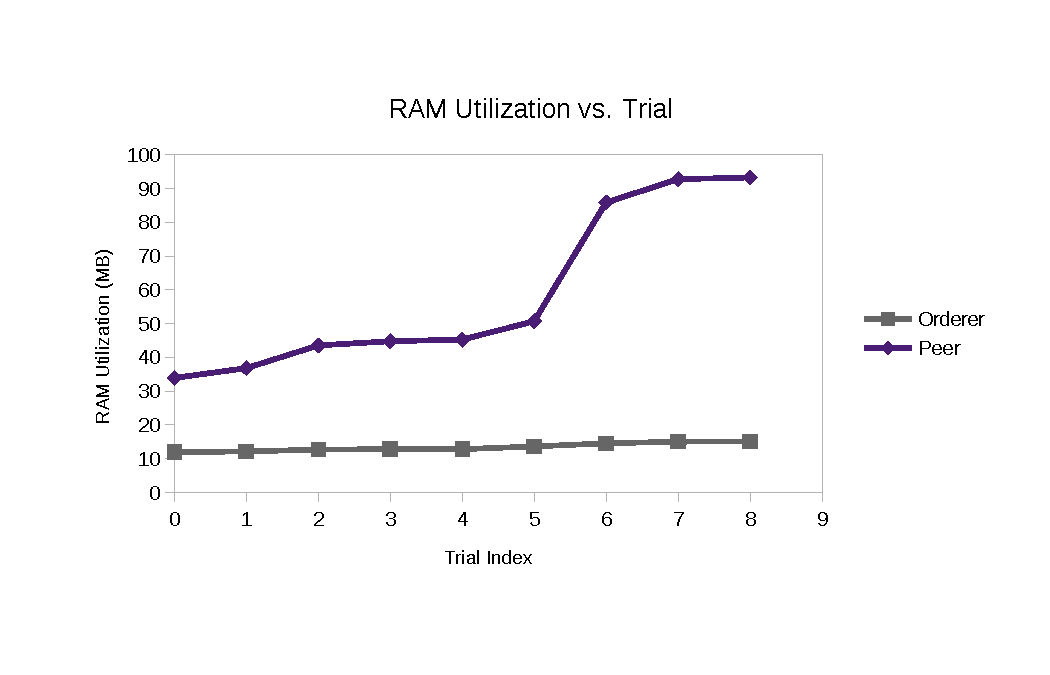
\includegraphics[width=\columnwidth]{ram-big}
  \vspace{-4em}
  \caption{RAM utilization appears correlated with the volume of
    transactions which have occurred, not the current transaction
    rate. This is consistent with ram usage being dominated by an
    in-memory cache.}
  \label{ram}
\end{figure}

Relatedly RAM utilization was difficult to measure cleanly. While I
expected the system's ram consumption to increase with the rate of
transactions, it actually increased linearly with the \emph{total
  volume} of transactions (see Figure \ref{ram}). This makes sense given the model of a ram
cache of database pages, but leads to a ram utilization curve steadily
climbing to the cache limit and eventually plateauing. I never
encountered the limit during my testing, so RAM utilization continued
to increase with each test run.

Given the compute bound nature of the distributed ledger processing
protocol, CPU utilization offers a clear picture of the system's performance.

\begin{figure}[t] 
  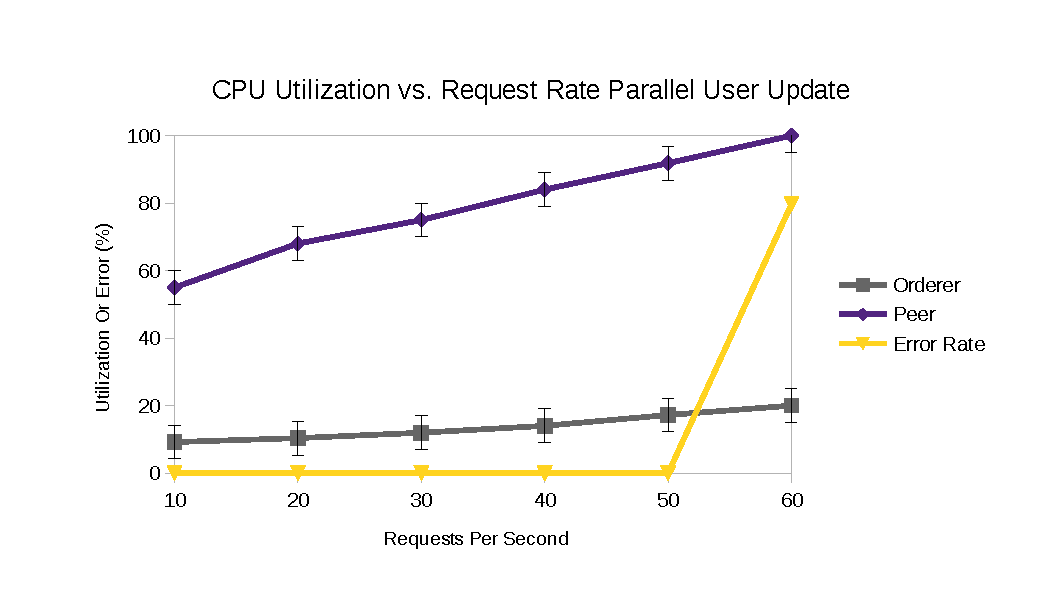
\includegraphics[width=\columnwidth]{parallel-utilization-big}
  \vspace{-2em}
  \caption{CPU utilization and error rate when updating multiple
    users' CRDTs in parallel. CPU utilization is proportional to the
    request rate.}
\end{figure}

\begin{figure}[t]
  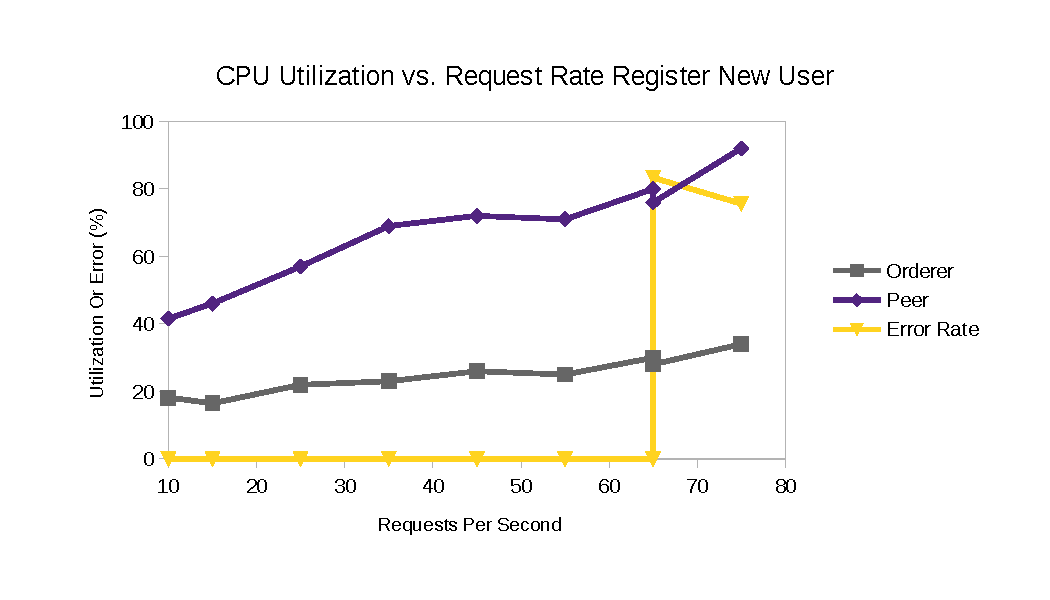
\includegraphics[width=\columnwidth]{new-user-big}
  \vspace{-2em}
  \caption{CPU utilization and error rate when registering many new
    users in parallel. CPU utilization is proportional to the request
    rate.}
\end{figure}

The high level error rate eventually spikes as the ledger system
saturates on CPU, is unable to handle all requests in time, and eventually
starts timing out. In my test cases generated from continuous flows of
synthetic data, handling the timeout increases the time elapsed of
future cases, leading to a cascading and easy to detect abort. Future
production versions of the queue manager could mitigate this behavior
through better admission control procedures.

\begin{figure}[t] 
  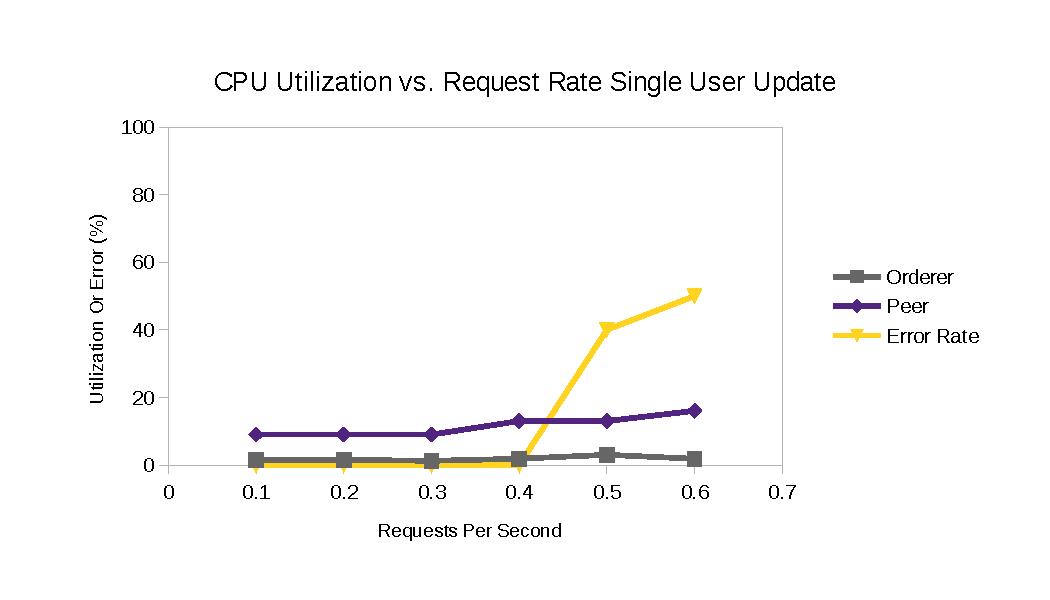
\includegraphics[width=\columnwidth]{single-user-big}
  \vspace{-2em}
  \caption{CPU utilization and error rate for updates to a single
    user. Single user updates are limited by the throughput provided
    by the optimistic concurrency control mechanisms built into the
    distributed ledger. Read/Write set conflicts are detected and
    transactions are aborted as the inter-transaction time for a
    single record dips below the amount of time required to execute a
    single transaction.}
  \label{single}
\end{figure}

Unlike when modifying different accounts, appending records to a
single CRDT is limited by the actual latency of committing a request
to the distributed ledger (see Figure \ref{single}). As the time
between transactions decreases below this latency, the optimistic
concurrency control mechanisms built into Hyperledger start to break
down and conflicts begin to occur. The observed rate of two seconds
per transaction is sufficient for the use case of a community network
call recording system though, and updates can reasonably be limited to
once every thirty seconds.

Lastly I measured the actual network I/O required per transaction on
the backhaul link. Using Wireshark I captured a trace of all IP
traffic generated during a single transaction on the backhaul link,
and measured the total IP payload size. Each transaction requires
300B, which is consistent with the size of the messages involved and
is sufficiently small to enable operation over a constrained satellite
link.

\section{Future Work}

While this initial class project delivered a promising proof of
concept prototype, much work and research remains to make it a usable
system. Essential missing components of the system are usage of a
robust encryption and signature verification library and the
incorporation of a persistent database to store queued records on the
basestation. Performance metrics in the distributed system will also
change as the number of peer nodes in the system varies, which I will
need to characterize by repeating measurements with a variable number
of peer nodes operational in the network. The docker based
implementation of the network should allow me to increase the number
of participating nodes with a cloud based container service, but I did
not get to setup a large scale test in time for the end of the
quarter.

Additionally, to keep the system incentive compatible, matching queue
and upload software must be deployed to the users' handsets. This
could come in the form of an STK sim application or a smartphone
application. SIM applications have the advantage of being transparent
to the user and accessible from the network, but expose a much more
limited programming environment. My lab is exploring exactly what
kinds of computation can occur in a SIM application and hopes to
deploy the user queuing software there.

Relying on a private chain for scalability means that users must have
the ability to understand the behavior of the network, admit new
members, and kick out bad actors. This is a difficult set of concepts
to visualize in an intuitive manner, and will be the subject of future
work.

Lastly a rich area of future exploration centers around co-optimizing
a distributed ledger for CRDTs. Techniques to address concurrent
updates with different data to the same user's CRDT could be as simple
as changing the layer at which writes are deconflicted or as
complicated as sharding and re-arranging how the CRDT is stored in the
ledger.

\subsection{Challenges}

The biggest challenges for me were related to learning how to develop
in the Hyperledger environment and learn how the fabric framework
exposes different ledger concepts. Hyperledger fabric is relatively
new, so while there are some tutorials available, they are not very
mature and documentation is actively under development. Having
overcome these challenges during the course of the course, I'm excited
to actually get time to polish the system and get it in a usable state
for deployment.

\section{Conclusion}

While I started this class project skeptical of whether a distributed
ledger would work in this context, I was pleasantly surprised by how
well my naiive prototype implementation scaled. I'm excited to
continue development and think this could be a viable approach for the
design of a federated community cellular network core.

%%% Local Variables:
%%% mode: latex
%%% TeX-master: "main"
%%% End:
